In this chapter, we introduce a version of the classical Euclidean norm PMCLP, where each facility has a given coverage radius. 
We refer to this problem as \sigla{MCD}{Maximum Covering by Disks}. We also propose an algorithm for it to later adapt it for the elliptical PMCLP in the next chapter. 

\section{Definition}

An instance of MCD is given by a set of $n$ demand points $\Pp:=\{p_1, \dots, p_n\}$, with $p_j\in\R^2$; a set of weights $\Ww:=\{w_1, \dots, w_n\}$, with $w_j\in\R_{\ge0}$ being the weight of point $p_j$; and $m$ disks given by their radii $\Rr:=\{r_1, \dots, r_m\}$, with $r_j\in\R_{>0}$. 
Additionally, to make the text more clear, we define a set of $m$ disks as $\D:=\{D_1, \dots, D_m\}$, with $D_j : \R^2 \mapsto \R^2$ being a function that takes the center where the $j$-th disk is located as input, and returns its coverage region as defined by \autoref{eq:disk}.

A solution for an instance of MCD is determined by $Q:=(q_1, \dots, q_m) \in \R^{2m}$, which specifies the center of every disk in $\D$. Let $w: 2^{\Pp} \mapsto \R_{\ge0}$ be a function, which takes a subset of $\Pp$ and returns the sum of the weights of every point in it, defined as

\begin{equation}\label{eq:subset_w}
w(A) = \sum_{j : p_j \in A} w_j.
\end{equation}
Then an optimal solution of MCD is formulated as a solution of

\begin{equation*}
\max_{Q} w\left(\bigcup_{j=1}^m \Pp \cap D_j(q_j)\right).
\end{equation*}

It is worth mentioning that MCD is a slightly different PMCLP than the one introduced in the first study on the subject in \citeonline{church:1984}. There, a coverage radius is given for each demand, rather than for each facility, and a demand point is considered covered if a facility is located within its radius.

\subsection{CLS and CIPS}

The method proposed in \citeonline{church:1984} involves the construction of a finite set of locations where each facility can be placed as a way of transforming a problem, where every point in $\R^2$ is a possible solution, into one where only a finite number of possibilities need to be considered. This set of possible locations is called \sigla{CLS}{Candidate List Set}.

In \citeonline{church:1984}, a CLS is set to be the \sigla{CIPS}{circle intersection point set}, which contains the intersection of circles with fixed radii centered at every demand point. This approach provides an optimal solution if a complete search on the CLS for every facility is done. 

We introduce, in this chapter, a $\bigO(n^2\lg{n})$ algorithm that returns a CLS for each facility, which is based on the idea presented in \citeonline{church:1984} and in the works for the one disk case by \citeonline{chazelle:1986} and \citeonline{cabello:2006}. We refer to the CLS for the $j$-th facility as $S_j$ and prove that, indeed, an optimal solution can be found by just considering the centers in $S_j$ for each facility.

\section{Related Work}
In \citeonline{cabello:2006}, a $\bigO(n^{2m-1}\log{n})$ algorithm for $MCD$ is developed as a sub-routine for its $(1-\epsilon)$-approximation algorithm. Firstly, they solve a sub-problem for two disks in $\bigO(n^3\log{n})$. Then, for the rest of the points that are not in that solution, it uses the algorithm developed in \citeonline{chazelle:1986} for the one-disk case, checking every possible solution for every one of the disks left.

Also, in \citeonline{zhou} an heuristic method for large-scale $MCD$ is proposed. It uses a probabilistic algorithm called mean-shift which is a gradient ascent method proven to converge to a local density maxima of any probability distribution. The mean-shift is utilized to find good candidates of centers for the unit disks, then the method backtracks to find the best assignment. The results showed that the greedy algorithm achieves an optimal coverage in some instances, but for some other ones it has a 15 percent worse coverage ratio.

\section{One disk version}

This version of the problem will be refered to as \sigla{MCD1}{Maximum Covering by One Unit Disk} and it is just a specific case of MCD with only one disk with radius one ($m=1$ and $r_1=1$). We refer to an instance of MCD1 as the tuple $(\Pp, \Ww)$.
We later use the algorithm for MCD1 here described to construct a CLS which is guaranteed to contain an optimal solution for MCD.

Two exact methods for MCD1 have been found in the literature. A $\bigO(n^2)$ algorithm is proposed by \citeonline{chazelle:1986} which improved the previously $\bigO(n^2\log{n})$ one proposed by \citeonline{drezner}.
As it has been mentioned, MCD1 is a 3SUM-HARD problem, which means that it is as hard as the 3SUM problem (the problem of finding three real numbers that sum to zero, given $n$ real numbers). Initially the lower bound of the 3SUM problem was conjectured to be $\Omega(n^2)$, matching the best algorithm for MCD1, which meant that no better time-complexity could be achieved. Since then, however, better algorithms for 3SUM have been developed with a $\bigO(\frac{n^2}{poly(n)})$ run time complexity \cite{3SUM-kopelowitz:2014}.


In \citeonline{drezner}, the main idea used to develop the $\bigO(n^2\log{n})$ algorithm is that, even though there are infinitely many points where the disk could be placed, only a few of them, a finite amount of $\bigO(n^2)$, needs to be considered for the method to find an optimal solution.
The algorithm, for every point, sorts the other points with respect to the angle they form with the first one. After that, the first point is placed on the border of the disk and, going through the sorted list, the algorithm inserts and removes points from the disk coverage. Also, when inserting and removing a point from the coverage, it only checks the disk centers that make the entering/leaving point to be on the border. Because the algorithm only checks the centers that make the disk have two points on its border, the number of centers it goes through is bounded by the number of pairs of points, which is $\binom{n}{2} = \bigO(n^2)$.

The algorithm for MCD1, developed in this chapter, can be seen as a parallel version of the algorithm developed by \citeonline{drezner}.
We, however, based on \citeonline{chazelle:1986} and \citeonline{cabello:2006}, decided to work with an equivalent problem called \sigla{MWC}{Maximum Weight Clique} which is introduced in the next section.

\section{Maximum Weight Clique}

An instance of the \sigla{MWC}{Maximum Weight Clique} is given by a list of points \mbox{$\Pp:=\{p_1,\dots,p_n\}$}, with $p_i \in \R^2$ representing the center of a unit disk;  and \mbox{$\Ww:=\{w_1, \dots, w_n\}$}, with $w_i\in \R_{>0}$ being the weight of the $i$-th unit disk. We also define a list $\D=\{D_1, \dots, D_n\}$, such that $D_i$, $i\in\{1,\dots,n\}$, is a unit disk centered at $p_i$ having weight $w_i$ assigned to it.

A clique, in this context, is a non-empty intersection region of one or more disks, and its weight is the sum of the weights of those disks in the intersection.
Following this, a solution for MWC can be defined as just a point $q\in\cup_{j=1}^n D_j$, which is inside any of the given disks in $\D$.
From a solution $q$, the corresponding clique $S$ can be obtained by intersecting every disk that contains $q$ as follows

\begin{equation*}
S = \bigcap_{j : q \in D_j} D_j.
\end{equation*}

With a geometric observation, though, the number of possible values for the solution can be reduced.
Let $\partial \D = \{ \partial D_1, \dots, \partial D_n \}$ be the set of circles corresponding to each disk in $\D$. 
Unless a clique is formed by only one disk, its boundary contains at least two points, which are the intersection of two circles that are part of the clique.
Because of that, $q$ can be limited to the set of pairwise intersections of $\partial \D$ as well as the set of centers of each disk $\Pp$, which considers the case where the optimal clique is composed of only one disk. With this observation, an optimal solution of MWC can be defined by the optimization problem

\begin{equation*}
\max_{q} \sum_{D_k \cap q \neq \emptyset} w_k,
\end{equation*}
with $q \in \{\partial D_i \cap \partial D_j : 1 \le i < j \le n\} \cup \Pp$. With this new specification of the solution's search space, given an instance of MWC, an optimal solution can be found by going through $\binom{n}{2} + n$ points, that is, $\bigO(n^2)$ points.

It is worth pointing out that MWC is a different problem than the maximum clique on a intersection graph (a graph where the vertices are the disks and an edge exists if there is an intersection between two disks). 
As shown in \autoref{fig:three_disks_no_intersection}, three disks could have non-empty pairwise intersection and still have an empty intersection of all of them together.
That is why MWC is also referred to as the Maximum Geometric Clique Problem and the other version, when there is only the pairwise intersection condition, is referred to as the Maximum Graphical Clique Problem \cite{inplace:2014}. 

%The graphical version of the problem was studied by \citeonline{graphical-clique}, where a $\bigO(n^{4.5})$ algorithm was proposed. Also, in \citeonline{inplace:2014}, a $\bigO(n^2\log{n})$ time in-place algorithm\footnote{An in-place algorithm is an algorithm that needs $\bigO(1)$ extra space.} for arbitrary radii disks was proposed. 

In \citeonline{chazelle:1986}, the method for MWC consists on building a planar graph on which the vertices are the $\binom{n}{2}$ pairwise intersection of the circumferences and the edges are the arcs of the circumferences connecting the intersections. With the graph constructed, a traversal is done to obtain the answer, thus the time complexity of $\bigO(n^2)$.

As it has been mentioned, with the equivalence of the two problems, an optimal solution of the Maximum Weight Clique Problem is also an optimal solution of MCD1, which means that a disk centered at $q^*$ which is an optimal solution of MWC, will have a maximal weight covering of the demand set $\Pp$.

Given an instance of MCD1, the equivalent MWC intance is obtained by defining the set $\D$ to contain the disks centered at $\Pp$ and setting the weight of every disk to be the weight of its corresponding point in $\Pp$. A disk $D_i$ will represent the area where a disk can be placed in order to cover $p_i$. This means that an intersection between some disks is a region where a disk could be placed to cover the corresponding points.

In \autoref{fig:three_disks_no_intersection}, it can be seen that there is no point where a disk could be placed such that it would cover $p_1, p_2$ and $p_3$, nonetheless, in any of the pairwise intersections, a disk could be placed to cover the two corresponding points.

\begin{figure}[h]
	\centering
	
	\caption{Three disks that have non-empty pairwise intersection among them, but no common intersection.}
	
	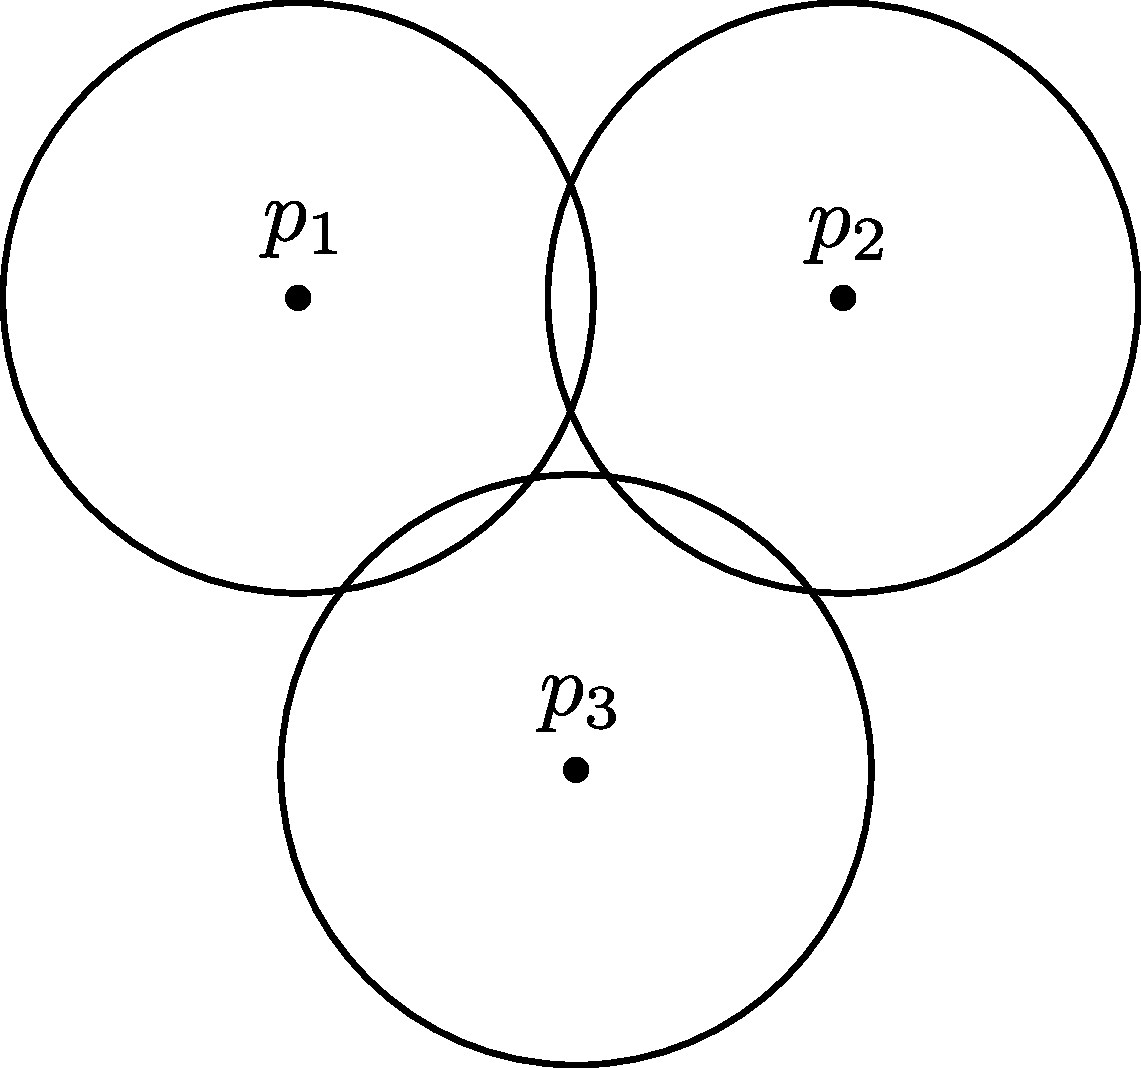
\includegraphics[scale=.25]{tex/figures/three_disks_no_intersection.pdf}
	\label{fig:three_disks_no_intersection}
	\fautor
\end{figure}

Formally, in MWC, if a point $q$ lies inside $\bigcap_{k \in I} D_k$, with $I \subset \{1,\dots,n\}$, then a disk centered at $q$ will cover the points $p_k$, with $k\in I$ in the equivalent MCD1 instance. Conversely, the same applies for a disk placed at $q$ that covers points $p_k$, with $k \in I$ in the MCD1 instance. It means that $q$ will lie inside region $\bigcap_{k \in I} D_k$ in MWC.

\subsection{An algorithm for the Maximum Weight Clique Problem}

The algorithm described here is based on the one in \citeonline{drezner}, also with some ideas from \citeonline{inplace:2014} and \citeonline{cabello:2006}. It has a run time complexity of $\bigO(n^2\log{n})$ and uses $\bigO(n)$ of extra space. It is worth noting, though, that a $\bigO((n+K)\log{n})$ run time, with $K$ being the number of intersections, can be obtained by using the algorithm in \citeonline{bentley:1979} to find all the intersections among the $n$ circumferences.

In \citeonline{inplace:2014} an important observation is made about the intersection regions of disks. Given an instance of MWC, any clique formed by a subset of $\D$ is bounded by the arcs of circles that intersect with it. Also, those arcs have the intersection of circles as their end-points. This can be seen on \autoref{fig:3disks_intersect} where the cliques that $D_1$ is part of are bounded by $D_1$'s arcs which have its intersections with the other circles as end-points. Following this, a definition is presented to characterize the end-points of an arc bordering a clique.

\begin{definicao}\label{def:inter_arc}
    Let $D_i$ and $D_j$ be two unit disks with non-empty intersection, and \mbox{$(\theta_1, \theta_2) \in [0,2\pi)^2$} be the two angles that $\partial D_i$ and $\partial D_j$ intersect, with the condition that $(\theta_1,\theta_2)$ defines an arc (counter-clockwise order) of $D_i$ that is the border of $D_i \cap D_j$. Then, define $\Gamma_+(i,j) = \theta_1$ and $\Gamma_-(i,j) = \theta_2$. For convenience, if $D_i$ is tangent to $D_j$, then $\theta_1=\theta_2$; and if $i=j$, then $\Gamma_+(i, j)=0$ and $\Gamma_-(i,j)=2\pi$.
\end{definicao}

\begin{figure}
\centering

    \caption{Three disks and their intersection points.}
    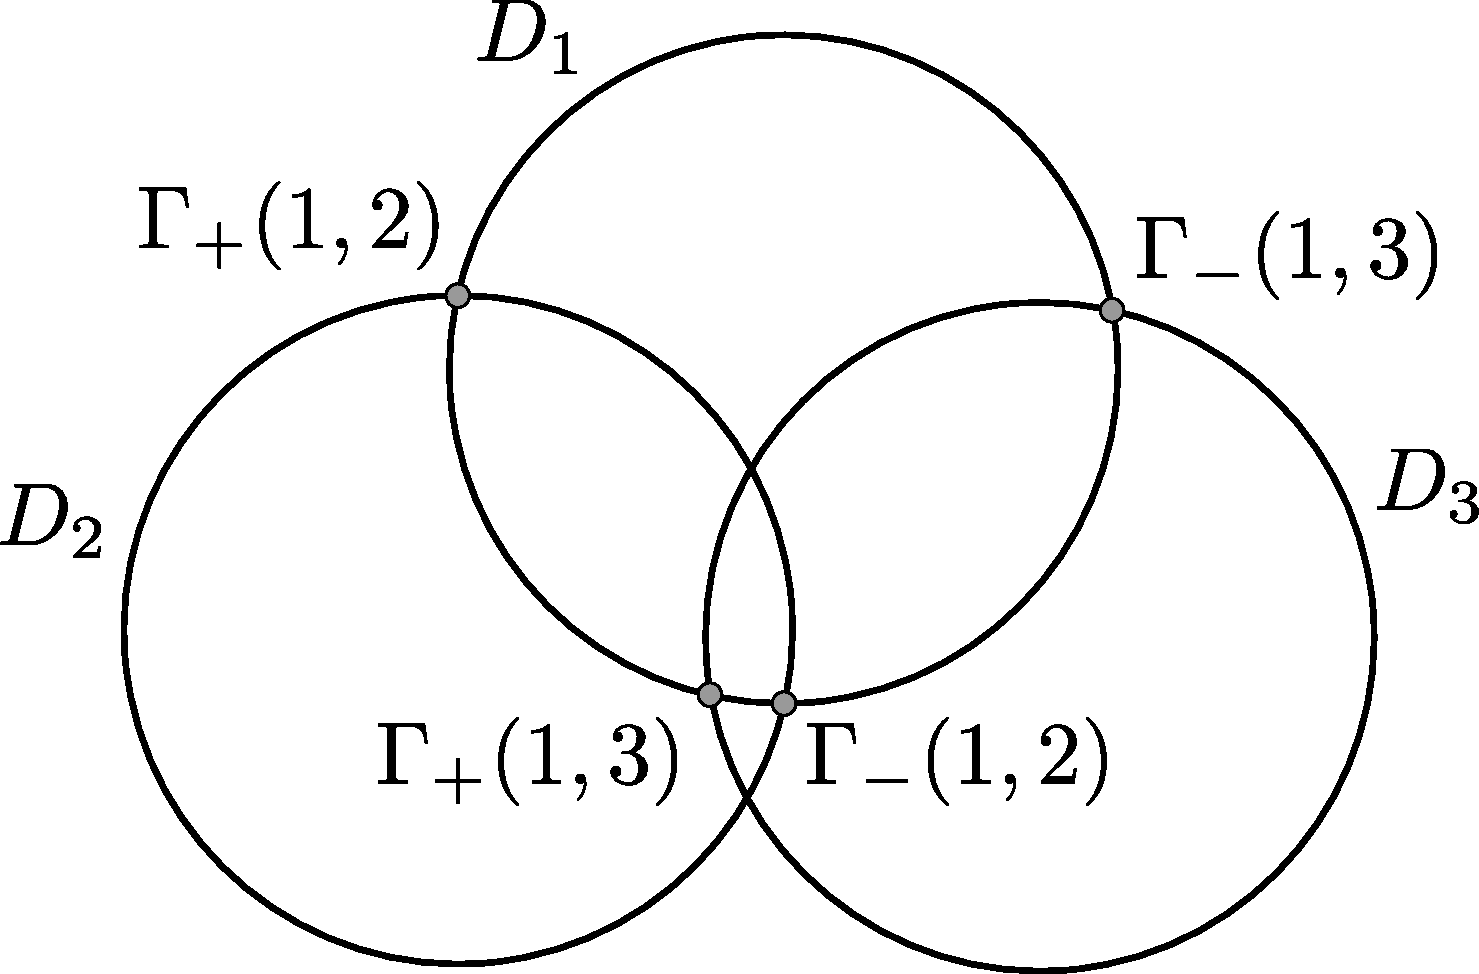
\includegraphics[scale=.3]{tex/figures/3_disks_intersect.pdf}
%    \begin{tikzpicture}
%\draw [help lines] (-5,-3) grid (5,3);

\draw[name path = c1] (0,0) circle (1cm);
\draw[name path = c3] (0.6,-0.82) circle (1cm);
\draw[name path = c2] (-0.4,-0.82) circle (1cm);

\node[above] at (0, 1) {$D_1$};
\node[left] at (-1.4, -0.82) {$D_2$};
\node[right] at (1.6, -0.82) {$D_3$};

\path [name intersections={of=c1 and c3}] ;
\foreach \i in {1,...,2}
\fill [color=gray] (intersection-\i) circle (2pt) ;

\node[right] at (intersection-1) {\tiny $\Gamma_-(1,3)$};
\node[left, below] at (intersection-2) {\tiny $\Gamma_+(1,3)$};

\path [name intersections={of=c1 and c2}] ;
\foreach \i in {1,...,2}
\fill [color=gray] (intersection-\i) circle (2pt) ;

\node[left] at (intersection-1) {\tiny $\Gamma_+(1,2)$};
\node[below,right] at (intersection-2) {\tiny $\Gamma_-(1,2)$};

%\draw [-] (-5,0) -- (5,0);
%\draw [-] (0,-3) -- (0,3);
%\draw [|-|] (0.001,-0.1) -- (4.999,-0.1);
\end{tikzpicture}
    \fautor
    \label{fig:3disks_intersect}
\end{figure}

Also, we refer to $\Gamma_+(i,j)$ as an opening angle, and to $\Gamma_-(i,j)$ as a closing angle. In \autoref{fig:3disks_intersect}, it is shown all the intersection points between $D_1$ with $D_2$ and $D_3$. Also, they are labeled according to \autoref{def:inter_arc}. Note that $\Gamma_+(1,3) > \Gamma_-(1,3)$ (the angles should be in the $[0,2\pi]$ interval).

With \autoref{def:inter_arc} in hand, we can establish the basis of the algorithm for MWC. For every disk $D_i$, let us describe an algorithm that gets the best clique which $D_i$ is part of. This way, an algorithm for MWC just uses that method for every disk and returns the best solution found. Firstly, let $A_i$ be a circular list that contains the intersection angles of $\partial D_i$ with every circle in $\partial \D$ defined as
\begin{equation*}
A_i = \bigcup_{j=1}^n \{ \Gamma_-(i,j), \Gamma_+(i,j) \}.
\end{equation*}
Assume also that $A_i$ is sorted in ascending order by the angle values with ties being broken by prioritizing opening angles.

Finding the best solution which $D_i$ is part of can be done by traversing $A_i$ while keeping a set of active disks. When an opening intersection angle is reached, the corresponding disk is added to the active set; and when a closing one is seen, the corresponding disk is removed from the active set. This way, finding an optimal solution can be achieved by keeping the weight of the active disks as well as the best clique found so far. Notice also that because $\Gamma_+(i,i)=0$ and $\Gamma_-(i,i)=2\pi$, any clique found by the traversal will also contain $D_i$.

In practice, traversing a circular list can be emulated by traversing a regular list that has a copy of the original circular list added to its end. 
Therefore, the list $B_i$ is defined here as a list that contains the elements of $A_i$ and a copy of it shifted to the interval $[2\pi, 4\pi]$. It is defined as

\begin{equation}\label{eq:b_i}
B_i = A_i\cup\bigcup_{j=1}^n \{ 2\pi+\Gamma_-(i,j), 2\pi+\Gamma_+(i,j) \}.
\end{equation}
Assuming $B_i$ is sorted with the same criteria as $A_i$, a simple traversal, starting at the first element and going until the last one, simulates a traversal on the circular list $A_i$.
This works because for any pair of disks $D_i$, $D_j$; $B_i$ contains $\Gamma_+(i,j) < \Gamma_-(i,j) + 2\pi$. That is, the algorithm encounters an opening angle before reaching a closing one for any circle.

In \autoref{fig:array_disks}, the intersection points between $\partial D_1$ (solid border) with $\partial D_2, \partial D_3$, and $\partial D_4$ (dashed border) are shown with a plus or minus sign indicating opening or closing intersection angles. 
The intersection list $B_1$ is also displayed in \autoref{fig:array_disks} along with the size of the set of active disks $Q$ after processing a point in $B_1$ -- this is exactly what \autoref{algoritmo:mcd_1} for MWC does for every disk. 
It is possible to see that the optimal clique highlighted in \autoref{fig:array_disks} is enclosed by the arcs defined by $\Gamma_+(1,4)$ and $\Gamma_-(1,4)$, and can also be identified by following $B_1$ while keeping track of $Q$.
The special intersection point of $\partial D_1$ with itself can also be seen in \autoref{fig:array_disks}. Its usage is very convenient as with $\Gamma_+(1, 1)$ and $\Gamma_-(1,1)$  in $B_1$, the algorithm inserts $D_1$ in the set of active disks before processing any point, and removes $D_1$ only after every point has been processed.
\begin{figure}[H]
	\centering
	
	\caption{The intersection list of a disk with three other disks.}
	%\usetikzlibrary{matrix}



\tikzset{every picture/.style={line width=0.75pt}} %set default line width to 0.75pt        

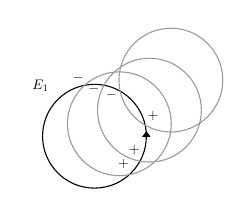
\begin{tikzpicture}[x=0.75pt,y=0.75pt,yscale=-1,xscale=1]
%uncomment if require: \path (0,95); %set diagram left start at 0, and has height of 95

%Shape: Circle [id:dp37777408295388804] 
\draw   (21,59.5) .. controls (21,45.69) and (32.19,34.5) .. (46,34.5) .. controls (59.81,34.5) and (71,45.69) .. (71,59.5) .. controls (71,73.31) and (59.81,84.5) .. (46,84.5) .. controls (32.19,84.5) and (21,73.31) .. (21,59.5) -- cycle ;
%Shape: Circle [id:dp4562198988843913] 
\draw  [color={rgb, 255:red, 155; green, 155; blue, 155 }  ,draw opacity=1 ] (47.5,46.94) .. controls (47.5,33.14) and (58.69,21.94) .. (72.5,21.94) .. controls (86.31,21.94) and (97.5,33.14) .. (97.5,46.94) .. controls (97.5,60.75) and (86.31,71.94) .. (72.5,71.94) .. controls (58.69,71.94) and (47.5,60.75) .. (47.5,46.94) -- cycle ;
%Shape: Circle [id:dp8913971633985722] 
\draw  [color={rgb, 255:red, 155; green, 155; blue, 155 }  ,draw opacity=1 ] (33,53.5) .. controls (33,39.69) and (44.19,28.5) .. (58,28.5) .. controls (71.81,28.5) and (83,39.69) .. (83,53.5) .. controls (83,67.31) and (71.81,78.5) .. (58,78.5) .. controls (44.19,78.5) and (33,67.31) .. (33,53.5) -- cycle ;
%Shape: Circle [id:dp05970043129919356] 
\draw  [color={rgb, 255:red, 155; green, 155; blue, 155 }  ,draw opacity=1 ] (57.81,32.47) .. controls (57.81,18.66) and (69,7.47) .. (82.81,7.47) .. controls (96.62,7.47) and (107.81,18.66) .. (107.81,32.47) .. controls (107.81,46.27) and (96.62,57.47) .. (82.81,57.47) .. controls (69,57.47) and (57.81,46.27) .. (57.81,32.47) -- cycle ;
%Straight Lines [id:da04725899028195979] 
%\draw[densely dotted]  (21,59.5) -- (71,59.5) ;


%Flowchart: Extract [id:dp5267407418119328] 
\draw  [fill={rgb, 255:red, 0; green, 0; blue, 0 }  ,fill opacity=1 ] (71,57.45) -- (72.52,59.55) -- (69.48,59.55) -- cycle ;

\draw (60,73) node [scale=0.5]  {$+$};
% Text Node
\draw (65.22,66) node [scale=0.5]  {$+$};
% Text Node
\draw (74.22,50) node [scale=0.5]  {$+$};
% Text Node
\draw (54.22,39.56) node [scale=0.5]  {$-$};
% Text Node
\draw (45.62,36.96) node [scale=0.5]  {$-$};
% Text Node
\draw (38.02,31.56) node [scale=0.5]  {$-$};


% Text Node
\draw (20,35) node [scale=0.5]  {$E_{1}$};
\end{tikzpicture}

\begin{tikzpicture}

\matrix [matrix of nodes,row sep=,row sep=0mm,
column 1/.style={nodes={rectangle,draw,minimum width=1.5em, minimum height=0.5em}},
column 2/.style={nodes={rectangle,draw,minimum width=1.5em, minimum height=0.5em}},
column 3/.style={nodes={rectangle,draw,minimum width=1.5em, minimum height=0.5em}},
column 4/.style={nodes={rectangle,draw,minimum width=1.5em, minimum height=0.5em}},
column 5/.style={nodes={rectangle,draw,minimum width=1.5em, minimum height=0.5em}},
column 6/.style={nodes={rectangle,draw,minimum width=1.5em, minimum height=0.5em}},
column 7/.style={nodes={rectangle,draw,minimum width=1.5em, color=gray, minimum height=0.5em}},
column 8/.style={nodes={rectangle,draw,minimum width=1.5em, color=gray, minimum height=0.5em}},
column 9/.style={nodes={rectangle,draw,minimum width=1.5em, color=gray, minimum height=0.5em}},
column 10/.style={nodes={rectangle,draw,minimum width=1.5em, color=gray, minimum height=0.5em}},
column 11/.style={nodes={rectangle,draw,minimum width=1.5em, color=gray, minimum height=0.5em}},
column 12/.style={nodes={rectangle,draw,minimum width=1.5em, color=gray, minimum height=0.5em}}
] (O)
{
$+$ & $-$ & $-$ & $-$ & $+$ & $+$ & $+$ & $-$ & $-$ & $-$ & $+$ & $+$\\
%$+$ & $-$ & $-$ & $-$ & $+$ & $+$\\
};

\node at (-4,-0.5) {$0$};
\node at (0,-0.5) {$2\pi$};
\end{tikzpicture}
	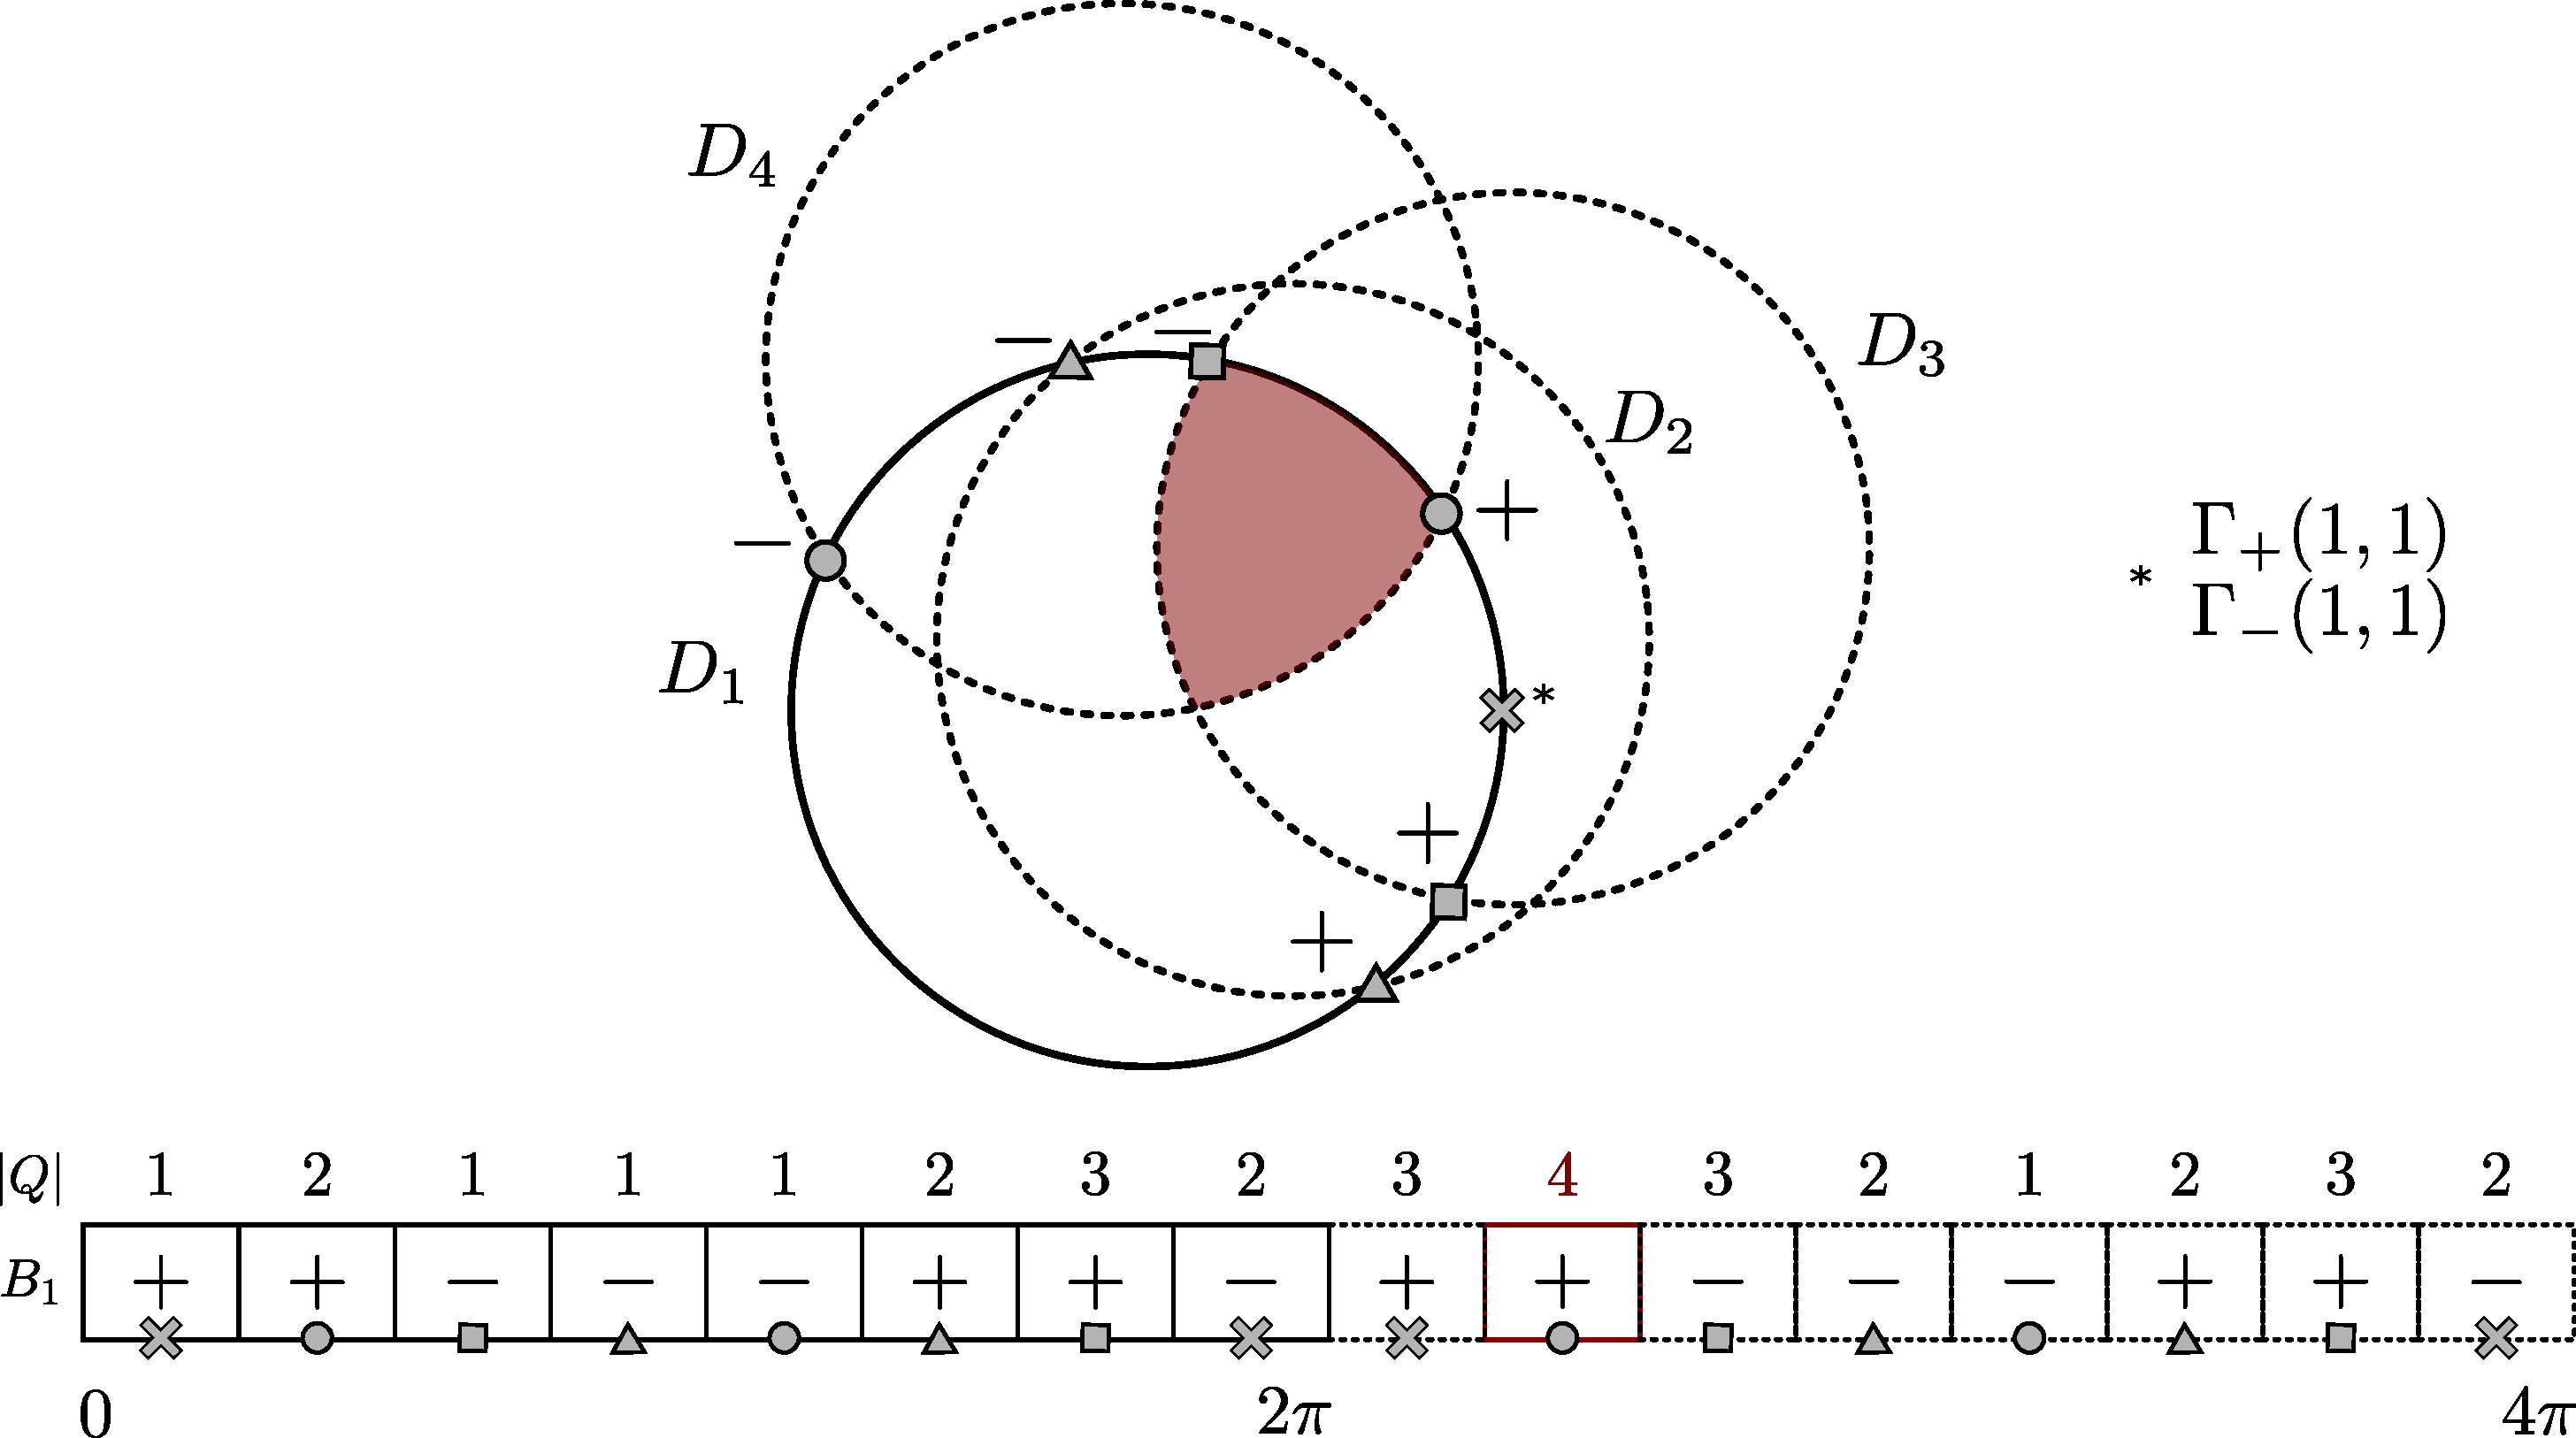
\includegraphics[scale=.3]{tex/figures/3_disks_intersect2.pdf}
	\fautor
	\label{fig:array_disks}
\end{figure}

Finally, we define \autoref{algoritmo:mcd_1} for MWC. Given an instance $(\Pp, \Ww)$ of MWC, the algorithm uses the approach described here of keeping a set of active disks while traversing the list $B_i$. It returns a point that is inside an optimal clique, this way \autoref{algoritmo:mcd_1} can also be used to get an optimal solution for an instance $(\Pp, \Ww)$ of MCD1.
\clearpage
\begin{algoritmo}[!htb]
	\caption{Algorithm for MWC.}\label{algoritmo:mcd_1}
	\begin{algorithmic}[1]
		\Require{A set of points $\Pp=\{p_1,\dots,p_n\}$, and a set of weights $\Ww=\{w_1, \dots, w_n\}$.}
		\Ensure{A point that is inside the maximum weight clique of unit disks.}
		
		\item[]
		
		\Procedure{$MWC$}{$\Pp, \Ww$}
		\State Let $\D=\{D_1, \dots, D_n\}$ be a set of unit disks, with centers in $\Pp$ and weights in $\Ww$
		
		\State $Q_{best} \gets \{\}$
		\State $q^* \gets$ $p_1$
		\ForAll{$D_i \in \D$}
		\State Let $B_i$ be the list of intersection angles of $D_i$ as defined by \autoref{eq:b_i}
		
		\State $Q \gets \{\}$ \Comment{The set of active disks.}
		\For{$\theta \in B_i$}\Comment{Assuming $B_i$ is sorted.}
		\State Let $D_j$ be the disk, such that $\theta \in D_j\cap D_i$
		\If{$\theta$ is a opening angle}
		\State $Q \gets Q \cup \{D_j\}$
		\Else
		\State $Q \gets Q \setminus \{D_j\}$
		\EndIf
		\If{$w(Q_{best}) < w(Q)$} 
		\State $Q_{best} \gets Q$
		\State $q^* \gets$ point corresponding to the intersection angle $\theta$
		\EndIf
		
		\EndFor
		\EndFor
		
		\State \Return $q^*$
		\EndProcedure
	\end{algorithmic}
\end{algoritmo}

\begin{theorem}\label{lema:disk}
	\autoref{algoritmo:mcd_1} for solving the Maximum Clique Problem has a $\bigO((n+K)\log{n})$ run time complexity, where $K$ is the number of intersections of the $n$ disks.
\end{theorem}

\begin{proof}
	Finding every intersection can be done in $\bigO((n+K)\log{n})$  by a plane sweep, the method is described in \citeonline{bentley:1979}. 
	Because sorting the intersection angles needs to be done, an additional $\bigO(K\log{K})$ pre-processing is added. All the other operations can be done in constant time. Therefore, the final algorithm complexity is $\bigO((n+K)\log{n})$.
\end{proof}

If a simpler implementation is desired, or the number of intersections is large, determining the set $I_i$ (the set of disks that intersect with $D_i$, defined in \autoref{algoritmo:mcd_1}) can be simply done in $\bigO(n^2)$, making the algorithm have a worst-case complexity of $\bigO(n^2\log{n})$.


\section{An algorithm for MCD}

A simple adaptation can be done on \autoref{algoritmo:mcd_1} to make it return a CLS that contains an optimal solution of MCD for that disk. This is shown in \autoref{algoritmo:mcd_cls}. 
Notice also that MCD1 is defined only for unit disks, however, this constraint can be dropped, as it is introduced just for the sake of keeping the text more simple and \autoref{algoritmo:mcd_1} works for any radius. A result about the runtime complexity of \autoref{algoritmo:mcd_cls} has already been given by \autoref{lema:disk}, the following result states about the adaption of it to be used in an algorithm for MCD.

\begin{lema}\label{lema:mcd}
	Suppose that an instance of MCD and an index $j\in\{1, \dots, m\}$ are given.
	Then \autoref{algoritmo:mcd_cls}, when given the instance $(\Pp, \Ww, r_j)$ as input, returns a CLS $S_j$ of size $\bigO(n^2)$, such that $q^*_j\in S_j$, with $(q^*_1, \dots, q^*_m)$ being an optimal solution of the given MCD's instance.
\end{lema}

\begin{proof}
It can be seen that in any solution of MCD, a disk placed at a point $q$ that covers at least one point $p \in \Pp$ has a correspondence to the Maximum Weight Clique Problem: the point $q$ is inside an intersection area of at least one disk and that area is bounded by some disk, which means it will be checked by \autoref{algoritmo:mcd_cls} as a candidate to be an optimal solution. The number of points \autoref{algoritmo:mcd_cls} goes through is $\bigO(n^2)$, then
obviously $|S_j|=\bigO(n^2)$.
\end{proof}

Then, with \autoref{algoritmo:mcd_cls}, an algorithm for MCD that checks every possible center for every disk yields a $\bigO(n^{2m})$ run-time complexity.
This algorithm is described in \autoref{chapter:ellipses} for the axis-parallel ellipses case.

It is worth mentioning that the choice of developing a different method for the problem, instead of using the one from \citeonline{cabello:2006}, is taken for the sake of simplicity, considering both algorithms achieve similar bounds.

\begin{algoritmo}
	\caption{Algorithm for MCD1 that returns a CLS.}\label{algoritmo:mcd_cls}
	\begin{algorithmic}[1]
		\Require{A set of points $\Pp=\{p_1,\dots,p_n\}$ with weights $\Ww=\{w_1, \dots, w_n\}$, and a radius $r\in\R_{>0}$.}
		\Ensure{A CLS for the disk given by radius $r$.}
		
		\item[]
		
		\Procedure{CLS-MCD}{$\Pp, \Ww, r$}
		\State $S \gets \{\}$
		\ForAll{$p_i \in \Pp$}
		%\State Let $D_i(p_i)$ be the disk with center at $p_i$
		\State Let $B_i$ be the list of intersection angles of $\partial D_i(p_i)$ as defined by \autoref{eq:b_i}
		
		\For{$\theta \in B_i$}\Comment{Assuming $B_i$ is sorted.}
		\If{$\theta$ is a opening angle}
		\State Let $q_\theta$ be the intersection point correspondent to angle $\theta$
		\State $S \gets S \cup \{q_\theta\}$	
		\EndIf
		\EndFor
		\EndFor
		
		\State \Return $S$
		\EndProcedure
	\end{algorithmic}
\end{algoritmo}